\section{High-Level Design}
\label{sec:highlevel}

The system has three major components: the tracking block, the gameplayme-play
block, and the glove block. The tracking block takes in video information from a
camera and estimates the x and y coordinates of the players hands. This
information is then passed to the gameplay block which models the physics of the
game, and outputs video information to the VGA display. The glove block contains
all off-chip circuitry, as well as the fpga hardware which controls the
vibration of the motors. See figure \ref{fig:high} for their major interactions.

\begin{figure}
\centering
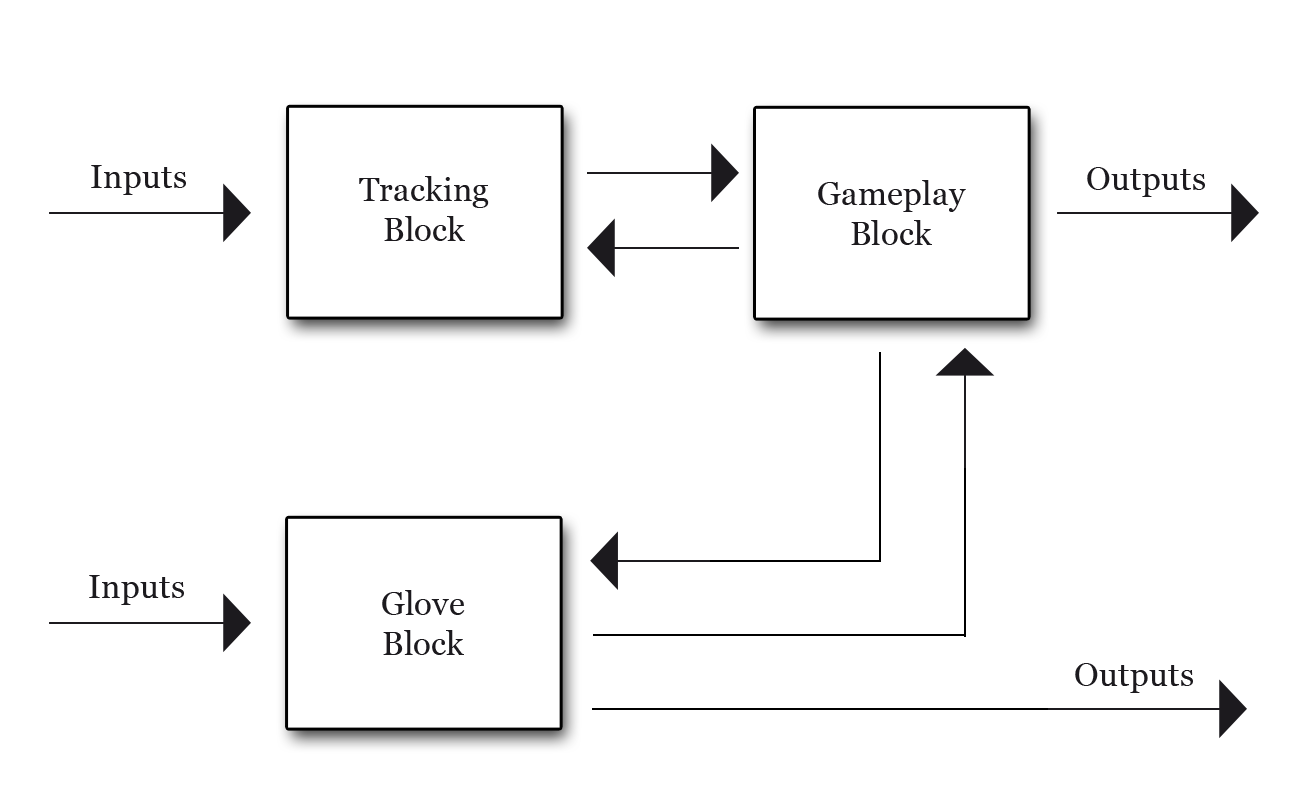
\includegraphics[scale=1]{img/high-level.png}
\caption{The virtual-reality rock climbing game is implemented with three major
components: the tracking block, the glove block, and the gameplay block.
Information flow is indicated with arrows. Note that input is processed by
either the glove or tracking system before being used by the gameplay block.}
\label{fig:high}
\end{figure}

\subsection{Tracking Block}

The tracking block analyzes video input from a camera and determines the
position of the players hands on screen. It takes color and ancillary
information as inputs and outputs the position of the players to the gameplay
block. This section was constructed by Turner Bohlen.

\subsection{Gameplay Block}

The gameplay block handles the physics of the game, and outputs video
informationmation to the VGA display. The gameplay block takes the hand position
from the tracking block as well as grab information from the glove block. From
this information, it determines the location of the player on the rock wall and
the handholds, the objects to display on screen, and whether or not the user is
grabbing a handhold. This section was constructed by Chris Lang.

\subsection{Glove Block}

The glove block comprises both the fpga and off-chip circuitry.  Its purpose is
to manage inputs to and outputs from the gloves. When a player flexes their hand
in real life, the off-chip circuitry signals the fpga, and the player grabs in
the game. Additionally, it takes information from the gameplay block describing
if the user is touching objects on screen and outputs a feedback signal to the
corresponding glove. This section was primarily constructed by Chris Lang,
although both partners were involved in its creation.
